%!TEX root = index.tex
\chapter{State of the art}
\section{Definitions}

Air Traffic Control service (ATC) can be devided into: area control service (ACC), approach control service (APP) and aerodrome control service (TWR) \cite[Chapter 1]{doc4444} The main objective is to prevent collisions between aircraft in air or on land and to expedite the flow of air traffic. \cite[Chapter 2.2]{annex11}
The airspace in which ATC service is provided can be divided into Control area (CTA), Control Zones (CTR) and Controlled aerodromes (TWR). Control area contains airways, terminal control areas and other airspace. It extends upwards from specified altitude. Within CTA, terminal control areas (TMA) are established to help in arrival and departure at some airports.
Control zones are normally situated below CTA and encompass airspace used by flights arriving at and departing from aerodromes. The diameter of CTR is at least 5NM in direction from which airplanes approach. CTR extends from the ground at least to the lower limit of CTA, but may extend further. CTR may include several aerodromes situated close together. \cite[Chapter 2.10]{annex11}

\begin{figure}[h]
    \centering
    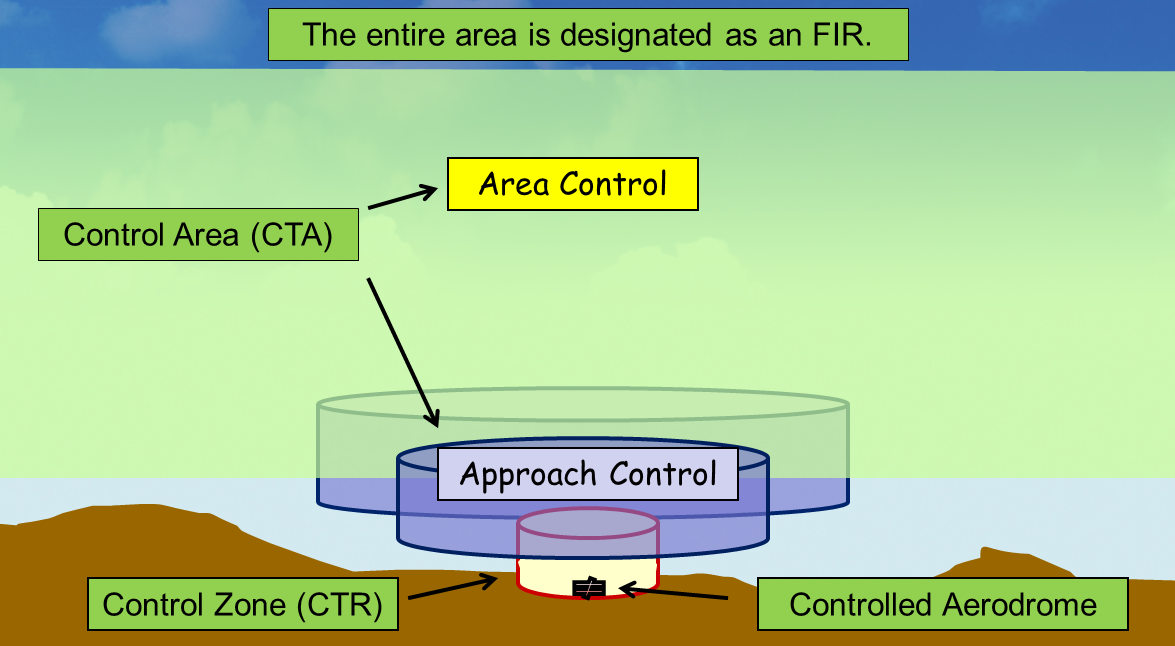
\includegraphics[width=0.8\textwidth]{figures/airspace.png}
    \caption{Airspace - \textcolor{red}{z prezentace 2011 ATM Lesson Plans/ATM 1-1 General Air Traffic Services podle \cite[Chapter 2.5]{annex11} - překreslit!}}
    \label{fig:airspace}
\end{figure}

\begin{figure}[h]
    \centering
    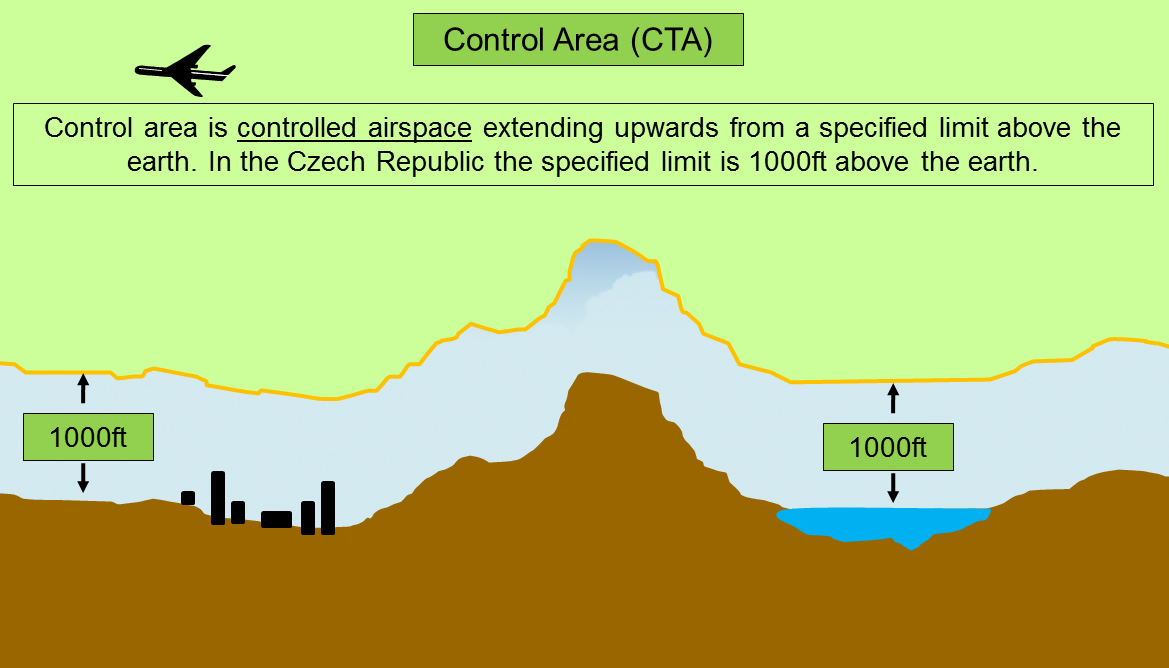
\includegraphics[width=0.8\textwidth]{figures/cta.png}
    \caption{CTA - \textcolor{red}{z prezentace 2011 ATM Lesson Plans/ATM 1-1 General Air Traffic Services podle \cite[Chapter 2.10]{annex11} - překreslit!}}
    \label{fig:cta}
\end{figure}

\begin{figure}[h]
    \centering
    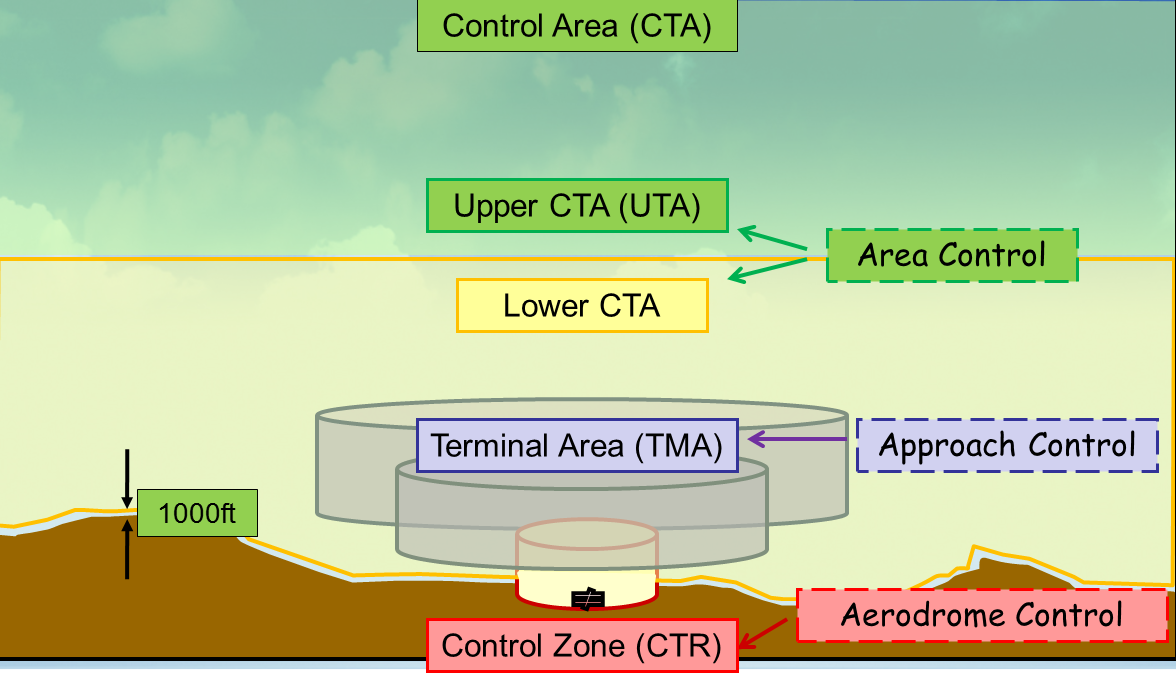
\includegraphics[width=0.8\textwidth]{figures/airspace2.png}
    \caption{Airspace - \textcolor{red}{z prezentace 2011 ATM Lesson Plans/ATM 1-2 General Air Traffic Control Service \cite[Chapter 2.10]{annex11} - překreslit!}}
    \label{fig:airspace2}
\end{figure}

\subsubsection{Area Control Service}
Area Control Service is an ATC service provided by area control centre (ACC) responsible for flights in Control Areas (CTA). Normally ACC is identified by the name of a nearby city, area or landmark. Smaller countries usually have one ACC, but many larger countries are controlled by several of them. ACCs usually control aircrafts in their en-route phase of flight. The ACC may be also responsible for flights to and from smaller aerodromes with no separate approach control service. \cite[Chapter 3.2]{annex11}

\subsubsection{Approach Control Service}
Approach Control Service (APP) is ATC service that is responsible for the part of CTA and CTR required by arriving or departing controlled flights (TMA). The primary functions of APP is sequencing arriving aircrafts and assisting departing aircrafts becoming established on course. The arrival and departure functions can be divided into several positions on busy aerodromes. APP is usually identified by the name of the aerodrome which it is serving, but sometimes it's not colocated with TWR and is at distant ACC location. When no separate ACC exists, approach control service is provided by ACC or TWR. \cite[Chapter 3.2]{annex11}

\subsubsection{Aerodrome Control Service}
Aerodrome control service is provided by a control tower (TWR) and is responsible for aircraft landing and taking off. It's also responsible for VFR flights in the CTR and for preventing collisions between aircrafts on the manoeuvring are of the aerodrome. \cite[Chapter 3.2]{annex11}

\textcolor{red}{z pohledu prostoru/z pohledu kontroly}

\textcolor{red}{v každou chvíli řídí letadlo jeden subjekt a místo a čas předání kontroly je jesně definované - kdy a jak?}

The controlled airspace can furthermore be classified as Class A-G. \cite[\textcolor{red}{kapitola}]{nolan} \textcolor{red}{popis jednotlivých classes podle nolana}

\textcolor{red}{Pro řízení v terminální oblasti nás zajímají všechny druhy řízení/prostoru, Agentfly má zatím jen ACC v CTA?}

\begin{figure}[h]
    \centering
    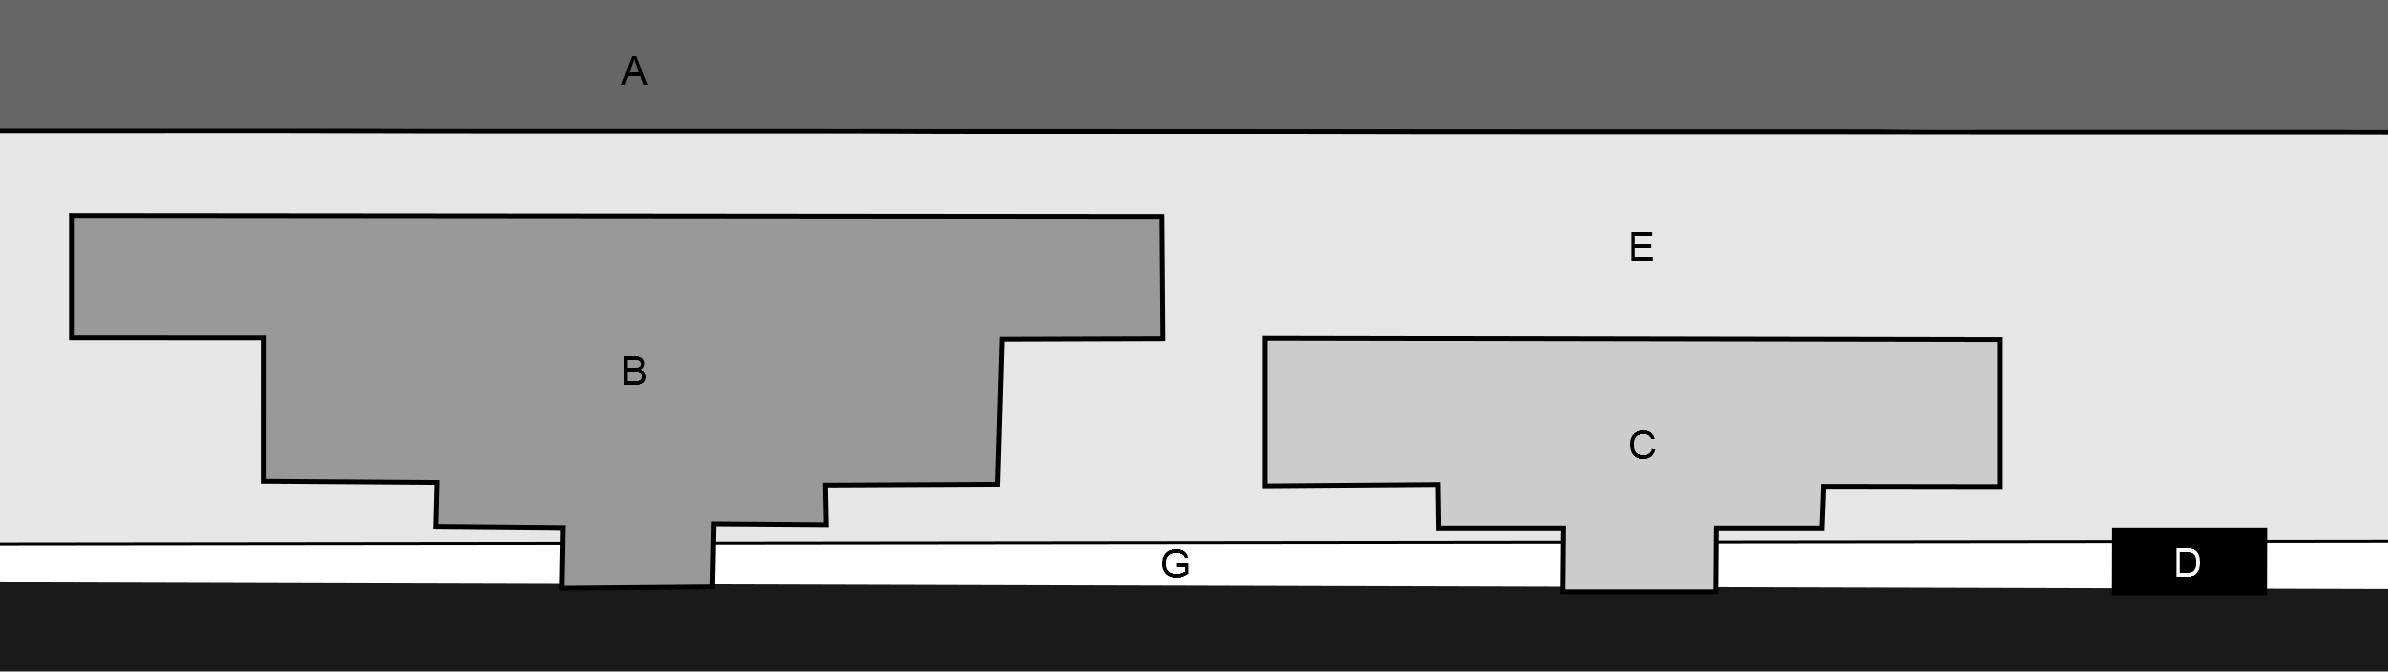
\includegraphics[width=0.8\textwidth]{figures/classes.png}
    \caption{Airspace Classification - \textcolor{red}{z prezentace 2011 ATM Lesson Plans/ATM 1-2 General Air Traffic Control Service \cite {nolan} - překreslit!}}
    \label{fig:classes}
\end{figure}

\textcolor{red}{SID a STAR routy?}

\subsubsection{Airspace Management}
ATM is generic term for any management activity for achieving the most eficient and flexible use of airspace avoiding permanent airspace segregation. \textcolor{red}{zdroj jen z prezentace}
The goals are to improve coordination between civil and military agencies, optimise route network and airspace structure and develop a free route airspace concept.

The concept of Flexible Use of Airspace (FUA) means that airspace should be treated as one continuous space that is being allocated according to user requirements. Any airspace segregation should only be temporary.

\subsubsection{Coordination within ATC}
unit $\leftrightarrow$ unit \\
ACC $\leftrightarrow$ APP \\
APP $\leftrightarrow$ TWR \\
sector $\leftrightarrow$ sector \\
sectors are within units

koordinaci mezi sektory popisuje \cite{doc4444} Doc 4444 Chapter 10
Detailed procedures are often subject to local regulations and rules.

Transferring unit/controller transfers the responsibility to control the aircraft to the accepting unit on point of transfer of control.

The transfer of control can be divided into three stages. First the flight is \bold{notified} to prepare for the transfer. Then the conditions of transfer of control are \bold{negotiated} with the transferring ATC unit and if necessary also with the accepting unit. After the parties \bold{agree}, the control is transferred to the accepting unit. his process can be achieved using automated means (AFTN, RDPS, FDPS, OLDI \textcolor{red}{?}) without using conventional telephone coordination. \textcolor{red}{(Jakože mezi sektory, s letadlem domluva asi pořád probíhá.)} \cite[Chapter 10.1.1]{doc4444}

This means that the flight is at any time under the control of only one ATC unit and can't be transferred from one unit to another without consent of the accepting unit. Also if communication with the aircraft is transwerred to the next unit, that unit cannot change the learance of the aircraft before the point of control transfer.

Doslovně z prezentace:
Control of an aircraft shall be transferred from ACC to APP, and vice versa, at a time or point agreed between the two units. This time or point is normally stated in a LOA.
Except when otherwise specified, APP may issue clearances to any aircraft released to it by ACC without reference to ACC. If an aircraft executes a missed approach, if necessary, ACC shall be informed immediately and subsequent action coordinated. 
After coordination with APP, ACC may release an arriving aircraft directly to TWR if the entire approach will be made under VMC.\cite[Chapter 10.1.3.1]{doc4444}

Doslovně z prezentace:
The take-off time is specified by the ACC when it needs to coordinate the departure with other ACC traffic or provide separation between other departing traffic on the same track. In other cases the APP determines the time of take-off so that the traffic in their AOR is separated. ACC and APP can also specify clearance expiry time if a delayed departure would cause separation problems. The time given by APP must not be later than ACC time. co je AOR?\cite[Chapter 10.1.3.2]{doc4444}

Doslovně z prezentace:
Exchange of movement and control data
APP shall keep ACC advised of data about controlled traffic such as:
RWY in use and type of instrument approach procedure;
lowest available level at the holding fix for use by ACC;
average time or distance intervals between successive arrivals as determined by APP;
revision of EATs as required (5 MIN or greater, or as agreed);
arrival times over holding fix when these vary by 3 MIN or greater from the times estimated by ACC;
flights cancelling IFR, if it will affect holding levels or EATs;
departure times, or if agreed, boundary or specified point times;
information relating to overdue or unreported aircraft; and
missed approach times which may affect ACC.
\cite[Chapter 10.1.3.3]{doc4444}

Doslovně z prezentace:
ACC shall keep APP advised of data about controlled traffic such as:
identification, type and point of departure of arrivals;
ETA and level of arrivals over holding fix or other specified point;
ATA and level of arrivals over holding fix if aircraft is released to APP after arriving over the holding fix;
requested type of instrument approach procedure if different to that specified by APP;
EAT issued;
when required, that an aircraft has been instructed to contact APP;
when required, that an aircraft has been released to APP, including if necessary, the time and conditions of release; and
anticipated delay to departures due to congestion.
ACC shall forward information on arrivals at least 15 MIN before ETA. \cite[Chapter 10.1.3.3]{doc4444}

Doslovně z prezentace:
Division of control
APP shall retain control of arrivals until the aircraft have been transferred to, and are in communication with TWR. Rules for transfer of control of arrivals shall be establish by LOAs or local instructions, considering airspace structure, terrain, MET conditions and ATS facilities available.
APP may authorize TWR to release a departure for take-off subject to the discretion of TWR with respect to arrivals.
TWR shall obtain approval from APP prior to authorizing SVFR flights, when so prescribed in LOAs or local instructions. \cite[Chapter 10.1.4.1]{doc4444}

Doslovně z prezentace:
Exchange of movement and control data
TWR shall keep APP advised of data about controlled traffic such as:
  arrival and departure times;
  when required, that the first aircraft in the approach sequence is in  	communication with and is sighted by TWR, and that reasonable 	assurance exists that a landing will be accomplished;
  information relating to overdue or unreported aircraft;
  information concerning missed approaches; and
  information concerning aircraft that are essential local traffic to aircraft 	under the control of APP.\cite[Chapter 10.1.4.2]{doc4444}


\textcolor{red}{konec 9-1 43}